\chapter{Code-breaking game model} \label{ch:model}

In this chapter, we formally define code-breaking games
  within the framework of propositional logic,
  where we represent a secret code as a valuation
  of propositional variables.
We define strategies in general, study several strategy classes and
  introduce \emph{one-step look-ahead strategies}.

\section{Notation and terminology} \label{sec:not}

Symbols $\Nseto$ and $\Nset$ denote the set of natural numbers with and without zero;
 the set of real numbers is denoted by $\Rset$.
The number of elements of a set $X$ is denoted by $|X|$.
Notation $X^* = \cup_{i\in\Nseto} X^i$ is used to denote the set of
  finite sequences of elements of $X$.
The $k$-th element of a sequence $s \in X^*$ is denoted by $s[k]$.

The set of all permutations of a set $\Var$ (bijections $\Var->\Var$)
  is denoted by $\Perm_\Var$ and
  $\idperm_\Var$ is the identity permutation.
A \emph{partition} $P$ of a set $X$ is a set of disjoint subsets of $X$,
  union of which is equal to $X$.
Members of $P$ are called \emph{cells}.
Let $P(x)$ be the cell containing $x$,
  i.e. $P(x) = A$, where $A\in P$ and $x\in A$.
For a function $f:X->Y$ and a set $Z\subseteq X$, the \emph{restriction of $f$ to $Z$}
  is denoted by $f|_Z:Z->Y$.


Let $\Form_\Var$ denote the set of \emph{propositional formulas} over
  the set of variables $\Var$ and let
  $\Val_\Var$ be the set of \emph{valuations} (boolean interpretations)
  of variables $\Var$.
Apart from standard logical operators, we allow $n$-ary \emph{numerical operators}
  $\exactlyk{k}\!$, $\atleastk{k}\!$, $\atmostk{k}\!$.
For a valuation $v\in\Val_\Var$ and propositional formulas
  $\form_1, ...,\form_n\in\Form_\Var$,
  the operator $\exactlyk{k}$ has the semantics
  $\val(\exactlyk{k}(\form_1,...,\form_n)) = 1$ if and only if
  $|\{i \| v(\form_i) = 1 \}| = k$.
The semantics of $\atmost$ and $\atleast$ is defined analogically.

Formulas $\form_0, \form_1 \in \Form_\Var$ are \emph{equivalent},
  written $\form_0 \equiv \form_1$, if
  $\val(\form_0) = \val(\form_1)$ for all $\val\in\Val_\Var$.
We say that \emph{$\val$ is a model of $\form$}
  or that \emph{$\val$ satisfies $\form$}
  if $\val(\form) = 1$.
For a formula $\form\in\Form_\Var$, let
  $\numval_{\!_\Var}{\form} = |\{ \val\in\Val_\Var \| \val(\form) = 1 \}|$
  be the number of models of $\form$.
We often omit the index $\Var$ if it is clear from the context.
A \emph{fixed variable} of a formula $\form$ is a
  variable that is assigned the same value in all models of $\form$.
If $\val(x) = 1$ for all $\val\in\Val$ such that $\val(\form)=1$, we say
that $x$ is fixed to 1 (or \emph{true}). Similarly, if $\val(x) = 0$, we say
that $x$ is fixed to 0 (or \emph{false}).

%-------------------------------------------------------------------------------
% DEF: CODE BREAKING GAME
\section{Basic definitions}

A code-breaking game can be represented by a \emph{set of variables},
  \emph{initial constraint} (a formula that is guaranteed to be satisfied),
  and a set of \emph{allowed experiments}.
An experiment is defined by the set of outcomes in which it can result.
The outcomes are specified in the form of a propositional formula that
  represents the partial information
  that the codebreaker gains if the experiment results in the outcome.

The number of experiments in a code-breaking game is typically very large.
For example, in the counterfeit coin problem defined in \autoref{s:coins},
  experiments correspond to combinations of coins you put on the pans of the
  balance scale.
It can be calculated that there are 36,894 combinations for 12 coins.
However, most of them have the same structure,
  so it would be inefficient to specify them one by one.
Therefore we have opted for a compact representation with \emph{parametrized experiments},
  where parametrization is a fixed-length string over a defined alphabet.
This whole idea is formalized below.

\begin{definition}[Code-breaking game] \label{def:game}
A \emph{code-breaking game} is a quintuple
  $\game = (\Var, \init, \Sigma, F, \Expt)$, where
  \begin{itemize}
  \item $\Var$ is a finite set of propositional variables,
  \item $\init \in \Form_\Var$ is a satisfiable propositional formula,
  %\item $\Expt$ is a finite set of types of experiments,
  \item $\Sigma$ is a finite alphabet,
  \item $F$ is a collection of mappings $\Sigma -> \Var$ with pairwise disjoint images,
  \item $\Expt$ is a set of \emph{parametrized experiments}, defined below.
  \end{itemize}
\vspace{8mm}
\end{definition}
\vspace{-15mm}
\begin{definition}[Parametrized experiment] \label{def:exp}
A \emph{parametrized experiment} for a game
  $\game = (\Var, \init, \Sigma, F, \Expt)$
  is a triple
  $\expt = (n, P, \outcome)$, where
  \begin{itemize}
  \item $n$ is the number of parameters of the experiment,
  \item $P$ is a partition of the set $\{1, ..., n\}$,
  \item $\outcome$ is a set of \emph{parametrized formulas}, defined below.
  \end{itemize}
Parameters of the experiment are elements of the alphabet $\Sigma$.
If $k$ and $l$ are in the same cell of the partition $P$, the $k$-th and
the $l$-th parameter must be different.
We denote the components of a parametrized experiment $t\in\Expt$
  by $n_t$, $P_t$, and $\outcome_t$.
\vspace{8mm}
\end{definition}
\vspace{-15mm}
\begin{definition}[Parametrized formula] \label{def-pform}
A \emph{parametrized formula} for a~parametrized experiment
$t$ of a game $\game = (\Var, \init, \Sigma, F, \Expt)$
  is a string $\pform$ generated by the following grammar, specified in Backus–Naur Form.
\begin{align*}
\msymb{form} &::= x \| f(\$k) \| \msymb{form} \circ \msymb{form} \| O(\msymb{form-list})  \| \neg\; \msymb{form},\\
\msymb{form-list} &::= \msymb{form-list} \;,\; \msymb{form} \| \msymb{form}
\end{align*}
  where $x\in\Var$ is a propositional variable, $f\in F$ is a mapping, $1<= k <= n_t$ is a parameter index,
  $\circ\in\{\wedge, \vee, ==>\}$ is a standard logical operator,
  and $O\in\{ \exactlyk{k}, \atmostk{k}, \atleastk{k} \| k\in\Nset\}$ is
  a numerical operator.
The special notation $\$k$ in $f(\$k)$ is used to denote the $k$-th parameter.
\end{definition}

The set $\Exp$ of all experiments in the game $\game$ is given by
\[
  \Exp =
     \big\{ (\expt, \param) \| t\in\Expt,\; \param \in\Sigma^{n_t},\;
     \forall x,y<={n_t}.\; P_t(x)=P_t(y) ==> \param[x] \not= \param[y] \big\}
\]

An experiment $e\in\Exp$ is thus a pair $(t, p)$, where
  $t$ is referred to as the \emph{type of the experiment},
 and $p$ is referred to as its \emph{parametrization}.

Let $e = (t, p)\in\Exp$ be an experiment,
  and $\pform\in\outcome_t$ a parametrized formula.
By $\pform(\param)$ we denote the application of
  the parametrization $\param$ on $\pform$,
  which is defined recursively on the structure of $\pform$
  in the following way:
\begin{align}
(x)(\param) &= x, \\
(f(\$k))(\param) &= f(\param[k]),\\
(\pform_1\circ\pform_2)(\param) &= \pform_1(\param) \circ \pform_2(\param),\\
O(\pform_1, ..., \pform_m)(\param) &= O(\pform_1(\param), ..., \pform_m(\param)),\\
(\neg\pform)(\param) &= \neg(\pform(\param)).
\end{align}

To simplify the notation, let us denote the set of outcomes of
  an experiment $\exp = (\expt, \param) \in \Exp$ by
  $\outcome(\exp) = \{ \pform(\param) \| \pform\in\outcome_\expt\}$.

\begin{example} \label{ex:run1}
Consider the counterfeit coin problem with 4 coins.
We use this game as a running example throughout this chapter.

The counterfeit coin and its relative weight to the others can be encoded
  as a valuation of variables $x_1, x_2, x_3, x_4$ and $y$,
  $v(x_i)$ being 1 if and only if the $i$-th coin is counterfeit and
  $y$ determining its relative weight
  ($v(y) = 0$ means that the counterfeit coin of underweight, $v(y) = 1$ means overweight).
The initial constraint $\init$ should capture the restriction that exactly one
  coin if counterfeit.
Therefore, let $\init$ be $\exactlyk{1}(x_1, x_2, x_3, x_4)$.

The experiments are parametrized by the coins on the pans of the balance scale.
Let $\Sigma = \{1, 2, 3, 4\}$ and $F = \{ f_x \}$ where $f_x$
maps the number $i$ to the corresponding variable $x_i$.

One parametrized experiment is weighing one coin against one, let us call it $t$.
We need two parameters ($n_t = 2$),
  the first determining the coin on the left pan and
  the second determining the coin on the right pan that must be different
  from the first.
$P_t$ is therefore the trivial partition $\{\{1, 2\}\}$.

If the left pan is lighter, it is either the case that the
  coin on the left is underweight ($f_x(\$1) \wedge \neg y$)
  or the coin on the right is overweight ($f_x(\$2) \wedge y$).
If the right pan is lighter, we get the symmetrical knowledge
  $(f_x(\$1)\wedge y) \vee (f_x(\$2)\wedge\neg y)$.
If both sides weigh the same, the counterfeit coins is not present on either pan
  and we can conclude $\neg f_x(\$1) \wedge \neg f_x(\$2)$.
To sum it up,
\begin{align*}
  t = \big(2,\; \big\{\{1,2\}\big\},\; \big\{ &
    (f_x(\$1)\wedge \neg y) \vee (f_x(\$2)\wedge y), \\
    & (f_x(\$1)\wedge y) \vee (f_x(\$2)\wedge\neg y), \\
    & \neg f_x(\$1) \wedge \neg f_x(\$2) \;\big\}\big).
\end{align*}

The second parametrized experiment is weighing two coins against two.
There are $4$ parameters, they must be pairwise distinct and the outcome
  formulas can be constructed analogically. \eqed
\end{example}


Note that the compact representation with parametrized experiments
  does not restrict the class of games that can fit \autoref{def:game},
  compared to a possible definition with direct experiment enumeration.
The reason is that there can always be a parametrized experiment
  with no parameters for each actual experiment.

\begin{definition}[Solving process]
An \emph{evaluated experiment} is a pair $(e, \form)$,
  where $e\in\Exp$ and $\form\in\outcome(e)$.
Let us denote the set of evaluated experiments by $\Omega$.

A \emph{solving process} is a finite or infinite sequence
  of evaluated experiments.
\end{definition}

For a solving process $\proc = (\exp_1, \form_1), (\exp_2, \form_2), ...$,
  let
\begin{itemize}
\item $|\proc|$ denote the length of the sequence,
\item $\proc(k) = \exp_k$ denote the $k$-th experiment,
\item $\proc[k] = \form_k$ denote the $k$-th outcome,
\item $\proc[1:k] = (\exp_1, \form_1), ..., (\exp_k, \form_k)$ denote the prefix of length $k$, and
\item $\aknow{\proc}{k} = \init \wedge \form_1 \wedge ... \wedge \form_k$
  denote the accumulated knowledge after the first $k$ experiments
  (including the initial constraint $\init$). For finite $\proc$,
  let $\tknow{\proc} = \aknow{\proc}{|\proc|}$ be the overall accumulated knowledge.
\end{itemize}

We denote the set of valuations that satisfy $\init$ by $\Vals = \{ \val\in\Val_\Var \| \val(\init) = 1 \}$
  and the set of \emph{reachable formulas} (formulas that represent some accumulated knowledge)
   by $\Formr = \{ \tknow{\proc} \| \proc\in\Omega^* \}$.

\subsection{Course of the game}

Let us now describe the course of the game in the defined terms.
\begin{enumerate} \itemsep -3pt
\item The codemaker chooses a valuation $\val$ from $\Vals$.
\item The codebreaker chooses an experiment $e$ from $\Exp$.
\item The codemaker gives the codebreaker a formula
  $\form\in\outcome(e)$ that is satisfied by the valuation $\val$.
  In order for the codemaker to always be able to do so,
  $\outcome(\exp)$ must contain a satisfied formula for every valuation in $\Vals$.
  This is defined below as \emph{well-formed} property of the game.
\item The evaluated experiment $(e, \form)$ is appended to the
  solving process $\proc$, which is initially empty.
\item If $\numval{\tknow{\proc}} = 1$, the codebreaker can uniquely determine
the valuation $\val$ and the game ends. Otherwise, it continues with step 2.
\end{enumerate}

\begin{definition}[Well-formed game] \label{def:wellformed}
A code-breaking game is \emph{well-formed} if for all $\exp \in \Exp$,
\begin{equation}
\forall\val\in\Vals.\;
  \exists \textrm{ exactly one }
     \form\in\outcome(\exp)\;.\; \val(\form) = 1
\end{equation}
\end{definition}

In the sequel, we focus only on well-formed games and
  we assume a given game is well-formed unless otherwise stated.

%-------------------------------------------------------------------------------
% EXAMPLE: FAKE-COIN PROBLEM
\subsection{Examples}
In the rest of this section, we show two ways of defining the counterfeit coin
  problem and a formal definition of Mastermind.
We do not provide formal definitions of other code-breaking games
  presented in \autoref{ch:games},
  however, a computer language for game specification
  that is based on this formalism is introduced in \autoref{ch:cobra},
  and specifications of all the code-breaking games
  in this language can be found in the electronic attachment to the thesis.

\begin{example}[The counterfeit coin problem] \label{ex:cc1}
A formal definition of the counterfeit coin problem with 4 coins
  has already been introduced in \autoref{ex:run1}.
This is a straightforward generalization for $n$ coins.
We define a game $\mathcal{F}_n = (\Var, \init, \Sigma, F, \Expt)$ with
the following components.

\begin{itemize}
\item
$\Var = \{x_1, x_2, ..., x_n, y\}$.
  Variable $x_i$ tells whether the $i$-th coin is counterfeit,
  variable $y$ tells whether it is lighter or heavier.
\item
$\init = \exactlyk{1}(x_1, ..., x_n)$,
  saying that exactly one coin is counterfeit.

\item
$\Sigma = \{1, 2,...,n\}$, $F = \{ f_x \}$, where $f_x(i) = x_i$.
The experiments are parametrized with coins that are represented by numbers from 1 to $n$.

\item
$\Expt = \big\{ (2\cdot m,\; \{\{1,...,2m\}\},\; \outcome_m) \| 1 <= m <= n/2 \big\}$, where
\begin{flalign*}
\outcome_m = \big\{
& ((f_x(\$1) \vee ... \vee f_x(\$m)) \wedge \neg y) \vee ((f_x(\$m+1) \vee ... \vee f_x(\$2m)) \wedge y), \\
& ((f_x(\$1) \vee ... \vee f_x(\$m)) \wedge y) \vee ((f_x(\$m+1) \vee ... \vee f_x(\$2m)) \wedge \neg y), \\
& \neg (f_x(\$1) \vee ... \vee f_x(\$2m)) \big\}.
\end{flalign*}

For every $m\in\Nset$, $m <= n/2$, there is a parametrized experiment of weighing
  $m$ coins against $m$ coins.
It has $2m$ parameters, the first $m$ are put on the left pan, the last $m$ are put on the right pan.

There are 3 possible outcomes.
First, the left pan is lighter.
  This happens if the counterfeit coin is lighter and it appears
  among the first $m$ parameters,
  or if it is heavier and it appears among the last $m$ parameters.
Second, analogically, the right pan is lighter.
Third, both pans weigh the same if the
  counterfeit coin does not participate in the experiment.
\end{itemize}

For demonstration purposes, we show another possible formalization
  of the same problem.
Let $\mathcal{F'}_n = (\Var, \init, \Sigma, F, \expt)$ be a game
  with the following components.

\begin{itemize}
\item
$\Var = \{x_1, x_2, ..., x_n,\: y_1, y_2, ..., y_n\}$.
Variable $x_i$ tells that the $i$-th coin is lighter, variable $y_i$ tells that the $i$-th coin is heavier.
\item
$\init = \exactlyk{1}(x_1, ..., x_n, y_1, ..., y_n)$,
  saying that exactly one coin is odd-weight.
\item $\Sigma = \{1, 2,...,n\}$, $F = \{ f_x, f_y \}$, where $f_x(i) = x_i$, $f_x(i) = y_i$.
\item
$\Expt = \big\{ (2\cdot m,\; \{\{1,...,2m\}\},\; \outcome_m) \| 1 <= m <= n/2 \big\}$, where
\begin{flalign*}
\outcome(w_m) = \big\{ & f_x(\$1) \vee ... \vee f_x(\$m) \vee f_y(\$m+1) \vee ... \vee f_y(\$2m), & \\
& f_y(\$1) \vee ... \vee f_y(\$m) \vee f_x(\$m+1) \vee ... \vee f_x(\$2m), & \\
& \neg\; (f_x(\$1) \vee ... \vee f_x(\$2m) \vee f_y(\$1) \vee ... \vee f_y(\$2m)) \big\}. &
\end{flalign*}
\end{itemize}
In this formalization, the variables correspond one-to-one to possible codes,
 so the outcome formulas effectively list all possibilities. \eqed
\end{example}

%-------------------------------------------------------------------------------
% EXAMPLE: MASTERMIND 2

\begin{example}[Mastermind] \label{ex:form-mastermind}
Mastermind game with $n$ pegs and $m$ colours can be formalized as
a code-breaking game
$\mathcal{M}_{n,m} = (\Var, \init, \Sigma, F, \Expt)$
  with the following components.

\begin{itemize}
\item
$\Var = \{x_{i,j} \| 1<=i<=n, 1<=j<=m \}$.
  Variable $x_{i,j}$ tells whether the $i$-th peg has the colour $j$.
\item
$\init = \bigwedge\left\{
  \exactlyk{1} \{x_{i,j} \| 1<=j<=m\} \| 1<=i<=n\right\}$, saying that
  there is exactly one colour at each position.
\item $\Sigma = \{1,...,m\}$, \\
 $F = \{ f_1, ..., f_n \}$, where $f_i(c) = x_{i,c}$ for $1<=i<=n$, \\
 $\Expt = \{ (n, P, \outcome) \}$.\\
There is only one parametrized experiment with $n$ parameters corresponding
  to the colours.
All parameters can be the same,
  so the partition $P$ is the discrete partition $\{\{1\},...,\{n\}\}$.
\item $\outcome = \{ \textsc{Outcome}(b, w) \| 0<=b<=n, 0<=w<=n, b+w<=n \}$,
where $\textsc{Outcome}$ is the function computed by the algorithm described below.
\end{itemize}

As described in \autoref{sec:mm},
  the outcome of an experiment in Mastermind corresponds
  to some maximal matching between
  the pegs in the code and the pegs in the guess.
The idea here is to generate a formula that asserts
  existence of such maximal matching
  with $b$ edges corresponding to black markers and
  $w$ edges corresponding to white markers.

The computation of \textsc{Outcome} $(b, w)$ is performed as follows.
First, we generate all admissible matchings.
Let $P = \{1,2,...,n\}$ be the set of positions.
\begin{itemize}
\item Select $B\subseteq P$ such that $|B| = b$.
  These are the positions at which the colour
  in the code matches the colour in the guess.
  They correspond to the black markers.
\item Select $W\subseteq P\times P$ such that $|W| = w$,
  $p_1(W)\cap B = \emptyset$, and $p_2(W)\cap B = \emptyset$,
  where $p_1$, $p_2$ are projections.
  These correspond to the white markers; $(i, j) \in W$ means that the colour
  at position $i$ in the guess is at position $j$ in the code.
\end{itemize}

Recall that $\inguess{i}$ represents the $i$-th peg in the guess
  and $\incode{i}$ represents the $i$-th peg in the code.
For a fixed combination $(B, W)$, we define a matching $M$ by
 $M = \{(\inguess{i}, \incode{i}) \| i\in B \} \cup
      \{(\inguess{i}, \incode{j}) \| (i, j)\in W \}$.
We construct a parametrized formula
  that asserts that $M$ is the maximal matching satisfying conditions in \autoref{sec:mm}
  for a guess $\$1,\$2,...,\$n$ and the code given by a valuation of the variables.
The formula has a form of a conjunction constructed in the following way.
\begin{itemize}
\item For $i\in B$, we add $f_i(\$i)$.
  This asserts that $(\inguess{i}, \incode{i})$ is an edge in the matching.
\item For $(i,j)\in W$, we add $f_j(\$i) \wedge \neg f_i(\$i) \wedge \neg f_j(\$j)$.
  This asserts that the colour $\$i$ is at position $j$ in the code and that
  $(\inguess{i}, \incode{i})$, $(\inguess{j}, \incode{j})$ are not edges
  in the matching.
\item For $(i,j)\in (P\setminus B\setminus p_1(W))
             \times (P\setminus B\setminus p_2(W))$, we add $\neg f_j(\$i)$.
  This asserts the matching is maximal as no edge can be added.
\end{itemize}

The result of $\textsc{Outcome}(b, w)$ is a disjunction
  of all the conjunctions constructed in this way
  for all combinations of $B$ and $W$.
For example, for $n = 4$, $B = \{1\}$ and $W = \{2, 3\}$, the generated formula is
\[ f_1(\$1) \wedge f_3(\$2) \wedge \neg f_2(\$2) \wedge \neg f_3(\$3)
  \wedge \neg f_2(\$3) \wedge \neg f_2(\$4) \wedge \neg f_4(\$3) \wedge \neg f_4(\$4). \]

The number of combinations for $B$ and $W$ grows exponentially
  with $n$ and so does the size of the generated formulas.
For $n = 4$, the result of $\textsc{Outcome}(1, 1)$
contains 24 clauses at the top level with 192 literals in total.\eqed

% For completeness, we show another way to formalize the Mastermind game,
%   which does not need algorithmic generation of the formulas.
% Let
%   $\mathcal{M'}_{n,m} = (\Var, \init, \Expt, \Sigma, \Exp, F, \outcome)$,
%   where

% \begin{itemize}
% \item $\Var$, $\init$, $\Sigma$, $F$ are defined as before.
% \item
% $\Expt = \{ g_{k_1,...,k_m} \| k_i \in \{1,...,n\}, \sum_ik_i = n \}$,\\
% $\Sigma = C$, \\
% $\Exp = \{(g_{k_1,...,k_m}, \param) \| \param\in\Sigma^{n},
%   \numpred{i}{\param[i]=j}=k_j\}$.\\
% The type $g_{k_1,...,k_m}$ covers all the guesses in which the number of $j$-coloured pegs is $k_j$.
% Therefore, two guesses for which we use the same pegs (pegs are just shuffled) are of the same type,
% but if we change a peg for one with different colour, it is other type of experiment.

% \item
% $F = \{ f_1, ..., f_n \}$, where $f_i(c) = x_{i,c}$ for $1<=i<=n$,
% \vspace{-2mm}
% \begin{flalign}
% \outcome(& g_{k_1,...,k_n}) =  \Big\{ &\\
%  & \exactlyk{b}\{ f_i(\$i) \| 1<=i<=n \} \;\wedge & \label{eq:mm-blacks}\tag{1}\\
%  & \exactlyk{t}\bigcup
%       \big\{
%            \{ \atleast{l}(x_{1,j},...,x_{n,j}) \| 1 <= l <= k_j \}
%            \| 1<=j<=m
%       \big\} & \label{eq:mm-whites}\tag{2}\\
%   &\hspace{2cm} \| 0<=b<=t, 0<=t<=n\Big\}.
% \end{flalign}
% \end{itemize}

% Part \eqref{eq:mm-blacks} of the formula captures the number of
%   the black markers.
% Part \eqref{eq:mm-whites} captures the total number of markers.
% Indeed, we get $k$ markers for colour $j$
%   if and only if $k < k_j$ and there are
%   at least $k$ pegs of colour $j$ in the code, i.e. all the formulas
%   $\atleast{i}(x_{1,j},...,x_{n,j})$ are satisfied for $i <= k$.
% Note that since the number of pegs of each colour is fixed by the type and we
%   do not care about the exact positions, this part of the formula
%   is not parametrized. \eqed
\end{example}

\section{Strategies in general}

This section introduces the concept of a strategy for experiment selection.
We define worst-case and average-case number of experiments of a strategy
 and optimal strategies. Further, we examine several strategy classes.

\begin{definition}[Strategy]\label{def:strategy}
A \emph{strategy} is a function $\stg: \Omega^* -> \Exp$,
  determining the next experiment for a given finite solving process.
\end{definition}

A strategy $\stg$ together with a valuation $\val\in\Vals$
  induce an infinite solving process
  \[
  \procstg{\stg}{\val} = \exp_1, \form_1, \exp_2, \form_2, ...,
  \]
  where
  $\exp_{i+1} = \stg(\exp_1, \form_1, ..., \exp_i, \form_i)$
  and
  $\form_{i+1}$ is the formula from $\outcome(\exp_{i+1})$
  satisfied by $\val$,
  for all $i\in\Nset$.
Note that thanks to the well-formed property,
  $\form_{i+1}$ is uniquely defined.

We define \emph{length} of a strategy $\stg$ on a valuation $\val$,
  denoted $\stglen{\stg}{\val}$,
  as the smallest $k\in\Nseto$ such that
  $\stgknow{\stg}{\val}{k}$ uniquely determines the code, i.e.
  \[
  \stglen{\stg}{\val} = \min \;\{ k\in\Nseto \| \numval{\stgknow{\stg}{\val}{k}} = 1 \}
  \]


The \emph{worst-case number of experiments} $\lenmax{\stg}$
  of a strategy $\stg$ is the maximal length of the strategy on a valuation $\val$,
  over all $\val\in\Vals$, i.e.
  \[
  \lenmax{\stg} = \max_{\val\in\Vals} \stglen{\stg}{\val}.
  \]

The \emph{average-case number of experiments} $\lenexp{\stg}$
  of a strategy $\stg$ is the expected number of experiments if the code
  is selected from models of $\init$ with uniform distribution, i.e.
  \[
  \lenexp{\stg} = \frac{
    \sum_{\val\in\Vals} \stglen{\stg}{\val}
    }{\numval{\init}}.
  \]

We say that a strategy $\stg$ \emph{solves the game} if $\lenmax{\stg}$ is finite.
Note that $\lenmax{\stg}$ is finite if and only if $\lenexp{\stg}$ is finite.
The game is \emph{solvable} if there exists a strategy that solves the game.

\medskip

\begin{definition}[Optimal strategy]
A strategy $\stg$ is \emph{worst-case optimal} if
  $\lenmax{\stg} <= \lenmax{\stg'}$ for any strategy $\stg'$.
A strategy $\stg$ is \emph{average-case optimal} if
  $\lenexp{\stg} <= \lenexp{\stg'}$ for any strategy $\stg'$.
\end{definition}

The following lemma provides us with a lower bound on the number of
experiments of a worst-case optimal strategy.

\begin{lemma} \label{lma:lbound}
Let $b = \max_{\expt\in\Expt} |\outcome(\expt)|$ be the maximal number of
  possible outcomes of an experiment. Then for every strategy $\stg$,
  \[
  \lenmax{\stg} >= \lceil \log_b(\numval{\init}) \rceil.
  \]
\end{lemma}

\begin{proof}
Let us fix a strategy $\stg$ and $k = \lenmax{\stg}$.
For an unknown model $\val$ of $\init$,
  $\stgknow{\stg}{\val}{k}$ can take up to
  $b^k$ different values.
By pigeon-hole principle, if $\numval{\init} > b^k$, there must be a valuation
  $v$ such that $\numval{\stgknow{\stg}{\val}{k}} > 1$.
This would be a contradiction with $k = \lenmax{\stg}$ and, therefore,
  $\numval{\init} <= b^k$, which is equivalent with the statement of the lemma.
  \qed
\end{proof}

\begin{lemma} \label{lma:accumulatedknowledge}
Let $\stg$ be a strategy and let $\val_1, \val_2 \in\Vals$.
If $\val_1$ is a model of $\stgknow{\stg}{\val_2}{k}$,
  then $\procstg{\stg}{\val_1}[1:k] = \procstg{\stg}{\val_2}[1:k]$.
\end{lemma}

\begin{proof}
Let $\proc_1 = \procstg{\stg}{\val_1}$, $\proc_2 = \procstg{\stg}{\val_2}$
and consider the first place where $\proc_1$ and $\proc_2$ differs.
It cannot be an experiment $\proc_1(i) \not= \proc_2(i)$ as they are both
  values of the same strategy on the same process:
$\proc_1(i) = \stg(\proc_1[1:i-1]) =
              \stg(\proc_2[1:i-1]) = \proc_2(i)$.

Suppose it is an outcome of the $i$-th experiment, $\proc_1[i] \not= \proc_2[i]$
  and $i <= k$.
Since $\val_1$ satisfies $\aknow{\proc_2}{k}$ and $i <= k$,
  it satisfies $\proc_2[i]$ as well.
However, $\val_1$ always satisfies $\proc_1[i]$ and
  both $\proc_1[i]$ and $\proc_2[i]$ are from the set
  $\outcome(\proc_1(i)) = \outcome(\proc_2(i))$.
Since there is exactly one satisfied experiment for each valuation in the set,
  $\proc_1[i]$ and $\proc_2[i]$ must be the same.
Contradiction. \qed
\end{proof}

\begin{example} \label{ex:run2}
Recall our running example of the counterfeit coin problem with 4 coins,
as defined in \ref{ex:run2}.

Consider a strategy $\stg$ defined as follows.
For simplicity, we denote experiments by their parametrizations only
  and the outcomes by a symbol $<$, $>$ and $=$,
  instead of the corresponding formula.
\[
\stg(\proc) = \left\{\begin{array}{ll}
13 & \textrm{ if } \proc = (12, <), \\
23 & \textrm{ if } \proc = (12, >),\\
14 & \textrm{ if } \proc = (12, =), (12, =), \\
34 & \textrm{ if } \proc = (12, =), (12, =), (14, =), \\
12 & \textrm{ otherwise.}
\end{array}\right.
\]

Let $\val\in\Vals$ be a valuation such that $v(x_3) = v(y) = 1$.
The induced solving process is
\[
\procstg{\stg}{\val} = (12, =), (12, =), (14, =), (34, >), (12, =), (12, =), ...
\]
The length of $\stg$ on $\val$ is 4, because $v$ is the only model of
  the accumulated knowledge after 4 experiments,
\[
\exactly_1(x_1,x_2,x_3,x_4) \wedge \neg(x_1 \vee x_2) \wedge \neg(x_1 \vee x_2)
\wedge \neg(x_1 \vee x_4) \wedge ((x_3 \wedge y) \vee (x_4 \wedge \neg y)).
\]

The strategy is intentionally inefficient and repeats the experiment $12$
if the outcome in the first step is `$=$'.
In fact, every valuation is discovered by $\stg$ in at most 4 experiments,
  so $\lenmax{\stg} = 4$.

\autoref{lma:lbound} gives us a lower bound $ \lceil\log_3(8)\rceil = 2$
 on the worst-case number of experiments of an optimal strategy.
However, we already know from \autoref{th:coins12} that the minimal number
  of experiments needed to reveal the code is 3.
\end{example}

\subsection{Non-adaptive strategies}

Non-adaptive strategies correspond to the well-studied problems of
  static Mastermind and
  non-adaptive strategies for
  the counterfeit coin problem\cite{mm-static}\cite{coins-nonadaptive}.
We define them here only to show the possibility of formulating the
  corresponding problems
  in our framework but we do not study them any further.

\begin{definition}[Non-adaptive strategy]
A strategy $\stg$ is \emph{non-adaptive} if it decides the next experiment
  based on the length of the solving process only, i.e.
  whenever $\proc_1$ and $\proc_2$ are processes such that
  $|\proc_1| = |\proc_2|$,
  then
  $\stg(\proc_1) = \stg(\proc_2)$.

Non-adaptive strategies can be considered functions $\stgx: \Nseto -> \Exp$,
where $\tau(|\proc|) = \stg(\proc)$.
\end{definition}

\subsection{Memory-less strategies}

The general definition of a strategy allows for the next experiment
  to depend on the exact history of the solving process,
  not only on the accumulated knowledge.
This is in a sense unintuitive, as
  the nature of code-breaking games is memory-less
  and the course of a game depends only on the accumulated knowledge.

\begin{definition}[Memory-less strategy]
A strategy $\stg$ is \emph{memory-less} if it decides the next experiment
  based on the accumulated knowledge only, i.e.
  whenever $\proc_1$ and $\proc_2$ are processes such that if
  $\tknow{\proc_1} \equiv \tknow{\proc_2}$
  then
  $\stg(\proc_1) = \stg(\proc_2)$.

Memory-less strategies can be considered functions
  $\stgx: \Formr -> \Exp$ such that
  $\form_1\equiv\form_2 ==> \stgx(\form_1)=\stgx(\form_2)$.
Then $\stg(\proc) = \stgx(\tknow{\proc})$.
\end{definition}

Note that the number of non-equivalent formulas over variable $\Var$
  is finite and, therefore, the number of memory-less strategies for a fixed
  code-breaking game
  is finite as well.

Now we prove some basic properties of memory-less strategies.
The following lemma says that once we do not get any new information
  from the experiment selected by a experiment,
  we never get any new information with the strategy.
Then, the theorem below proves that there exists an optimal
  memory-less strategy.

\begin{lemma}
Let $\stg$ be a memory-less strategy and $\val\in\Vals$.
If there exists $k\in\Nset$ such that
  $\numval{\stgknow{\stg}{\val}{k}} = \numval{\stgknow{\stg}{\val}{k+1}}$,
 then
  $\numval{\stgknow{\stg}{\val}{k}} = \numval{\stgknow{\stg}{\val}{k+l}}$
 for any $l\in\Nset$.
\end{lemma}

\begin{proof}
To simplify the notation, let $\know^k = \stgknow{\stg}{\val}{k}$.
There is a formula $\form\in\outcome(\know^k)$,
  such that $\know^{k+1} \equiv \know^{k} \wedge \form$.
Therefore, if $\know^{k+1}$ is satisfied by valuation $\val$, so must be $\know^{k}$.
Since $\numval{\know^{k}} = \numval{\know^{k+1}}$, the sets of
  valuations satisfying $\know^{k}$ and $\know^{k+1}$ are exactly the same
  and the formulas are thus equivalent.
This implies $\stg(\know^{k}) = \stg(\know^{k+1})$ and $\know^{k+2} \equiv \know^{k+1}\wedge \form \equiv \know^{k+1}$.

By induction,
  $\stg(\know^{k+l}) = \stg(\know^{k})$ and
  $\know^{k+l} \equiv \know^{k}$
  for any $l\in\Nset$.\qed
\end{proof}

\TODO{W-c vs A-c???}
\begin{theorem} \label{th:memless}
Let $\stg$ be a strategy.
Then there exists a memory-less strategy $\stgx$ such that
  $\stglen{\stg}{\val} >= \stglen{\stgx}{\val}$ for all $\val\in\Vals$.
\end{theorem}

\begin{proof}
Let us choose any total order $\form_1, \form_2, ...$ of $\Formr$ such that
  if $\form_i$ implies $\form_j$, then $i <= j$.
We build a sequence of strategies $\stg_0, \stg_1, \stg_2, ...$ inductively in the following way.
Let $\stg_0 = \stg$.
\begin{itemize}
\item If there is no $v\in\Vals, k\in\Nseto$ such that
  $\stgknow{\stg_{i-1}}{v}{k} \equiv \form_i$, select any $\exp\in\Exp$ and
  define $\stg_i$ by
\[
\stg_i(\proc) = \left\{
 \begin{array}{lll}
 \stg_{i-1}(\proc)  & \textrm{ if } \tknow{\proc}\not\equiv\form_i,\\
 \exp               & \textrm{ if } \tknow{\proc}\equiv\form_i.
 \end{array}
 \right.
\]
Clearly, all induced solving processes for $\stg_i$ and $\stg_{i-1}$ are the same
  and $\stglen{\stg_i}{v} = \stglen{\stg_{i-1}}{v}$.

\item If there exists $v\in\Vals, k\in\Nseto$ such that
  $\stgknow{\stg_{i-1}}{v}{k} \equiv \form_i$, choose the largest $l$ such that
  $\stgknow{\stg_{i-1}}{v}{l} \equiv \form_i$ and define
\[
\stg_i(\proc) = \left\{
 \begin{array}{lll}
 \stg_{i-1}(\proc)            & \textrm{ if } \tknow{\proc}\not\equiv\form_i,\\
 \procstg{\stg_{i-1}}{v}(l)   & \textrm{ if } \tknow{\proc}\equiv\form_i.
 \end{array}
 \right.
\]
First we prove that this definition is correct.
Let $v_1, v_2, k_1, k_2$ be such that
  $\stgknow{\stg_{i-1}}{v_1}{k_1}\equiv\form_i\equiv\stgknow{\stg_{i-1}}{v_2}{k_2}$.
Take $l_1, l_2$ as the largest numbers such that
  $\stgknow{\stg_{i-1}}{v_1}{l_1}\equiv\form_i\equiv\stgknow{\stg_{i-1}}{v_2}{l_2}$.
Since $v_1$ satisfies $\stgknow{\stg_{i-1}}{v_2}{l_2}\equiv\form_i$,
  then $\procstg{\stg_{i-1}}{v_2}[1:l_2] = \procstg{\stg_{i-1}}{v_1}[1:l_2]$
  by \autoref{lma:accumulatedknowledge}.
The same holds for $l_1$ which means that $l_1 = l_2$ and
  $\procstg{\stg_{i-1}}{v_1}(l_1) = \procstg{\stg_{i-1}}{v_1}(l_2)$, which
  proves that the definition of $\stg_i$ is independent of the exact choices
  of $v$ and $k$.

Now $\stglen{\stg_i}{v} = \stglen{\stg_{i-1}}{v} - (l-k)$, where
  $k$ and $l$ is the smallest and the largest number such that
  $\stgknow{\stg_{i-1}}{v}{k}\equiv\form_i $ and
  $\stgknow{\stg_{i-1}}{v}{l}\equiv\form_i $, respectively,
  because
  $\procstg{\stg_{i-1}}{v}(l) = \procstg{\stg_{i}}{v}(k)$ and due to the ordering,
  the rest of the process is independent of the beginning.
\end{itemize}

The last strategy of the sequence is clearly memory-less and satisfies the
  condition in the lemma. \qed
\end{proof}

% \begin{lemma}
% Let $b = \max_{\expt\in\Expt} |\outcome(\expt)|$ be the maximal number of
%   possible outcomes of an experiment.
% If for any $\form\in\Formr$,
% \[
%   \exists\exp . \max_{\formx\in\outcome(\exp)} \numval{(\form\wedge\formx)} =
%   \left\lceil \frac{\numval{\form}}{b} \right\rceil,
% \]
% then a greedy strategy $\stg$ is optimal and
% \[
%   \lenmax{\stg} = \lceil \log_b(\numval{\init}) \rceil.
% \]
% \end{lemma}

% \begin{proof}
% \TODO{Napsat důkaz.}
% \end{proof}

\begin{example}
Recall the game and the strategy $\stg$ from \autoref{ex:run2}.
The strategy is clearly not non-adaptive, as
  $\stg((12, <)) \not= \stg((12, >))$.
It is neither memory-less as
  $\stg((12, =)) \not= \stg((12,=),(12,=))$ but
  the accumulated knowledge of the solving processes is the same.

Consider a non-adaptive strategy
 $\stgx:\; 1 \mapsto 12,\; 2\mapsto 13,\; 3\mapsto 14$.
If the counterfeit coin is among the first three,
  it is discovered by the strategy in two experiments.
If the counterfeit coin is coin 4, it requires three experiments.
Hence $\lenmax{\stgx} = 3$ and the value of $\stgx$ on
  greater numbers is irrelevant.

If we apply the construction in \autoref{th:memless} on $\stg$,
we get a memory-less strategy $\stg'$, given by

\[
\stg'(\form) = \left\{\begin{array}{ll}
13 & \textrm{ if } \form \equiv (x_1 \wedge \neg y) \vee (x_2 \wedge y), \\
23 & \textrm{ if } \form \equiv (x_1 \wedge y) \vee (x_2 \wedge \neg y),\\
14 & \textrm{ if } \form \equiv \neg x_1 \wedge \neg x_2, \\
34 & \textrm{ if } \form \equiv \neg x_1 \wedge \neg x_2 \wedge \neg x_4, \\
12 & \textrm{ otherwise.}
\end{array}\right.
\]

Notice that the valuation $v$ with $v(x_3) = v(y) = 1$ is discovered in
  3 experiments as the strategy does not repeat the experiment 12 now.
Therefore, $\lenmax{\stg'} = 3$.

Both strategies $\tau$ and $\stg'$ are worst-case optimal. \eqed
\end{example}

\section{One-step look-ahead strategies} \label{sec:oslas}

Specification of a strategy in general can be very complicated.
In this section, we study a subclass of memory-less strategies that we call
  \emph{one-step look-ahead}.
These strategies select an experiment that
  minimizes the value of a given function
  on the set of possible knowledge in the next step.

\newcommand{\formset}{\Psi}
\begin{definition}[One-step look-ahead strategy]\label{def:oslas}
Let $f$ be a function of type $2^{\Formr} -> \Rset$.
A one-step look-ahead strategy with respect to $f$ is
  a memory-less strategy such that
  for every $\form\in\Form_X$ and $\exp'\in\Exp$,
\[
f(\{\:\form \wedge \formx \| \formx\in\outcome(e) \:\}) <=
  f(\{\: \form \wedge \formx \| \formx\in\outcome(e') \:\}).
\]
\end{definition}

Note that one-step look-ahead strategy with respect to $f$ is not unique.
For some formulas, there can be more experiments with the same value of $f$.
To uniquely specify a strategy, we must provide the function $f$ and
  a resolution method for these ambiguous states.
Typically, we specify a total order on experiments and select the least
  experiment in the order satisfying the condition of \autoref{def:oslas}.

A few one-step look-ahead strategies for Mastermind
  have been already introduced in \autoref{sec:mm}.
We now define them formally in the general code-breaking games.
In the Mastermind case,
  the experiments are ordered lexicographically by the colour combination.

\begin{description}
\item[Maximal number of models.]
This strategy minimizes the worst-case number of remaining codes.
For Mastermind, this was suggested by Knuth\cite{mm-knuth}.
\[
f(\formset) = \max_{\form\in\formset} \numval{\form}
\]

\item[Expected number of models.]
This strategy minimizes the expected number of remaining codes.
  For Mastermind, this was suggested by Irwing\cite{mm-expnum}.
\[
f(\formset) = \frac{\sum_{\form\in\formset}(\numval{\form})^2}{\sum_{\form\in\formset} \numval{\form}}
\]

\item[Entropy of the number of models.]
This strategy maximizes the entropy of the numbers of remaining codes,
For Mastermind, this was suggested by Neuwirth\cite{mm-entropy}.
\[
f(\formset) = \sum_{\form\in\formset} \frac{\numval{\form}}{N} \cdot \log \frac{\numval{\form}}{N}
  \textrm{, where } N = \sum_{\form\in\formset}\numval{\form}
\]

\item[Number of satisfiable outcomes.]
This strategy maximizes the number of possible outcomes.
For Mastermind, this was suggested by Kooi\cite{mm-mostparts}.
\[
f(\formset) = - \:|\{ \form \| \form\in\formset, \;\SAT{\form} \}|
\]
\end{description}

\newcommand{\fixed}{\#_\textrm{fixed}\:}
We suggest and analyse one-step look ahead strategies based on fixed variables.
Let
\[
\fixed\form = |\{ x\in\Var \| \forall v.v(\form)=1 ==> v(x)=1 \}
                  \cup\{ x\in\Var \| \forall v.v(\form)=1 ==> v(x)=0 \}|
\]
be the number of variables that have same value in all models of $\form$.
Note that while the aforementioned strategies does not depend on the exact
  formalization of a problem, the number of fixed variables may differ for
  different encodings.
For example, the choice of the following strategies in \autoref{ex:cc1} differs
  for the two possible formalisations.

\begin{description}
\item[Minimal number of fixed variables.]
\[
f(\formset) = -\min_{\form\in\formset} \fixed{\form}
\]
\item[Expected number of fixed variables.]
\[
f(\formset) = -\frac{\sum_{\form\in\formset}\numval{\form}\cdot\fixed{\form}}{\sum_{\form\in\formset}\numval{\form}}
\]
\end{description}

\begin{example}
Recall \autoref{ex:run1} and consider two experiments in the first step.

First, consider an experiment of weighing coin 1 against coin 2.
All the 3 outcomes are satisfiable, the number of models is
  2, 2 and 4 for outcome $<$, $>$, and $=$, respectively.
If the experiment results in $<$ or $>$, we know that the counterfeit coin
is coin 1 or coin 2. If it results in $=$, the counterfeit coin is coin 3 or coin 4.
Therefore, every outcome fixes two variables.

Second, consider an experiment of weighing coins 1 and 2 agains coins 3 and 4.
As exactly one coin must be counterfeit, outcome $=$ is not possible.
Outcomes $<$ and $>$ are symmetrical, both have $4$ models and fix no variables.

\autoref{tbl:run-oslas} shows the values of the defined
  strategies on these two experiments.
The experiment $12$ wins with all strategies except for Maximal number of models,
  where the values are the same.
\begin{table}[ht]
\begin{center}
\begin{tabular}{l|cc}
& 12 & 1234 \\\hline
Maximal number of models & 4 & 4 \\
Expected number of models & 3 & 4 \\
Entropy of the number of models & -1.04 & -0.69 \\
Number of satisfiable outcomes & -3 & -2 \\
Minimal number of fixed variables & -2 & 0 \\
Expected number of fixed variables & -2 & 0 \\
\end{tabular}
\caption{Values of various one-step look-ahead strategies on experiments 12 and 1234.}
\label{tbl:run-oslas}
\end{center}
\end{table}

\end{example}

% Greedy strategies are optimal in the fake-coin game $\mathcal{F}_n$.

% \TODO{Napsat důkaz.}



\chapter{Experiment equivalence and algorithms} \label{ch:expeq}

What makes the analysis of code-breaking games difficult is
  typically the large number of experiments.
For example, during the evaluation a one-step look-ahead strategy
  with respect to function $f$,
  we need to compute the value of $f$ on all experiments.
The number of experiments is even more important for optimal strategy synthesis,
  where we have to consider all possible experiments in every state
  and analyse whether the experiment can lead to an improvement
  of the number of experiments of a strategy.

Fortunately, some experiments are usually equivalent to some others in the sense
  that the knowledge they can give us is either exactly the same or symmetrical.
In the counterfeit coin problem, for example,
  the parametrized experiment of weighing 4 coins against 4 coins
  has $\frac{1}{2}\cdot {12 \choose 4}\cdot{8 \choose 4} = 17,325$
  possible parametrizations.
In the initial state, however,
  all of them are equivalent
  as they give us symmetrical knowledge.

%Algorithms for symmetry detection in Mastermind
%   based on graph isomorphism have been suggested in \cite{cbg-nauty}.

This chapter formally introduces the concept of experiment equivalence.
We prove that in various situations, it is sufficient to consider
  one experiment from each equivalence class.
This fact is used in the presented algorithms for well-formed check,
  evaluation of a one-step look-ahead strategies and
  optimal strategy synthesis.

\section{Experiment equivalence} \label{sec:expeq}

We start with a formal definition of equivalence of two experiments.
The section continues with our suggestion on a method for equivalence testing
  based on isomorphism of labelled graphs.
This method is crucial for the algorithms presented in the following sections.

\begin{definition}[Experiment equivalence] \label{def:expeq}
Let $\exp\in\Exp$ be an experiment and $\perm\in\Perm_\Var$ a variable permutation.
A $\perm$-symmetrical experiment to $\exp$ is an experiment
  $\exp^\perm\in\Exp$
  such that
  $\{\form^\perm \in\outcome(\exp)\} = \{\form\in\outcome(\exp^\perm)\}$.
Clearly, no $\perm$-symmetrical experiment to $e$ may exists.

A \emph{symmetry group} $\symg$ of a given game is
  the maximal subset of $\Perm_\Var$ such that for
  every $\perm\in\symg$ and $\exp\in\Exp$,
  there exists a $\perm$-symmetrical experiment to $\exp$.

Finally, an experiment $\exp_1\in\Exp$ is equivalent to $\exp_2\in\Exp$ with respect to $\form$,
  written $\exp_1\expeq{\form}\exp_2$,
  if and only if there exists a permutation $\perm\in\symg$ such that
 \[ \{ \form\wedge\formx \| \formx\in\outcome(\exp_1) \} \equiv
   \{ (\form\wedge\formx)^\perm \| \formx\in\outcome(\exp_2) \}. \]
\end{definition}

\begin{example}
Recall the running example from the previous chapter, introduced in \autoref{ex:run1}.
Experiment 23 is a $(x_1x_3)$-symmetrical experiment to 12, because for $\perm = (x_1x_3)$,
\begin{alignat*}{5}
\big\{ \;(&(x_1 \wedge \neg y) \vee (x_2\wedge y))^\perm,\;
   (&&(x_1 \wedge y) \vee (x_2\wedge\neg y))^\perm,\;
   (&&\neg (x_1  \vee x_2))^\perm \;\big\} = \\
\big\{ \;&(x_3 \wedge \neg y) \vee (x_2\wedge y),
   &&(x_3 \wedge y) \vee (x_2\wedge\neg y),
   &&\neg (x_3 \vee x_2)\; \big\}.
\end{alignat*}

In fact, for every experiment $e = (t, p)$ and every permutation $\perm$ stabilizing $y$,
  we can permute the parameters of $t$ accordingly and get a $\perm$-symmetrical experiment to $e$.
Therefore, the symmetry group $\symg$ is $\{\perm\in\Perm_\Var \| \perm(y) = y\}$.

Since $\symg$ is also the symmetry group of $\init$,
  all experiments of the same type are equivalent,
  and the quotient set of $E$ by $\expeq{\init}$
  has only two equivalence classes.
For a more complex example, let $\form = \init\wedge\neg(x_1\vee x_2)$.
Experiment $3124$ is now equivalent to $43$, with $\perm = \idperm_\Var$.
The corresponding formulas are equivalent even though they
  are syntactically different. \eqed
\end{example}

In the rest of the section, we suggest a method for testing
  whether two given experiments are equivalent with respect to a given formula.

First, we show a construction of the \emph{base graph} for a given game,
  automorphisms of which are a subset of the symmetry group $\symg$.
Then we describe the construction of the \emph{experiment graph} for a given experiment,
  which is build on top of the base graph.
  We prove
  that if the experiment graphs are isomorphic,
  the corresponding experiments are equivalent.

Recall that a \emph{labelled graph} is a triple $(V, E, l)$, where
  $(V, E)$ is a graph and $l: V->L$
  is a labelling function ($L$ being a set of labels).
Isomorphism of two labelled graphs is a bijection between their sets of vertices
that preserves edges and labels.

\subsection{Base graph construction}

The base graph for a game $\game = (\Var, \init, \Sigma, F, \Expt)$ is a labelled graph $B = (V,E,l)$ described below.
\begin{itemize}
\item There is a vertex for every proposition variable and every mapping, i.e. $V = \Var \cupdot F$.
\item A mapping is connected by edges with all variables in its value range, i.e. $(f, x) \in E$ if there is a symbol $a\in\Sigma$ such that $f(a) = x$,
\item Two variables are connected by an edge if they are values
  of different mappings on the same symbol of the alphabet,
  and these mappings appear in outcome formulas of the same parametrized experiment.
  Formally, $(x_1, x_2) \in E$ if there is a symbol $a\in\Sigma$ and mappings
  $f_1,f_2\in F$ such that $f_1(a) = x_1$, $f_2(a) = x_2$, and
  there is a parametrized experiment $t\in T$ and a number $k <= n_t$ such that
  both $f_1(\$k)$ and $f_2(\$k)$ appear in the outcome formulas of the
  parametrized experiment $t$.
\item
  The vertices corresponding to mappings have their own labels.
  The vertices corresponding to variables are labelled ``variable'',
  expect for the variables that appear directly in some outcome formula
  of a parametrized experiment. These have their own labels as well.
\end{itemize}

\begin{example} \label{ex:cc-runbase}
The base graph for the counterfeit coin problem with 4 coins is shown in
\autoref{fig:base-graph} on the left.
Note that vertices $y$ and $f_x$ have separate labels while
  other vertices are labelled ``variable''.

\begin{figure}[ht]
\begin{center}
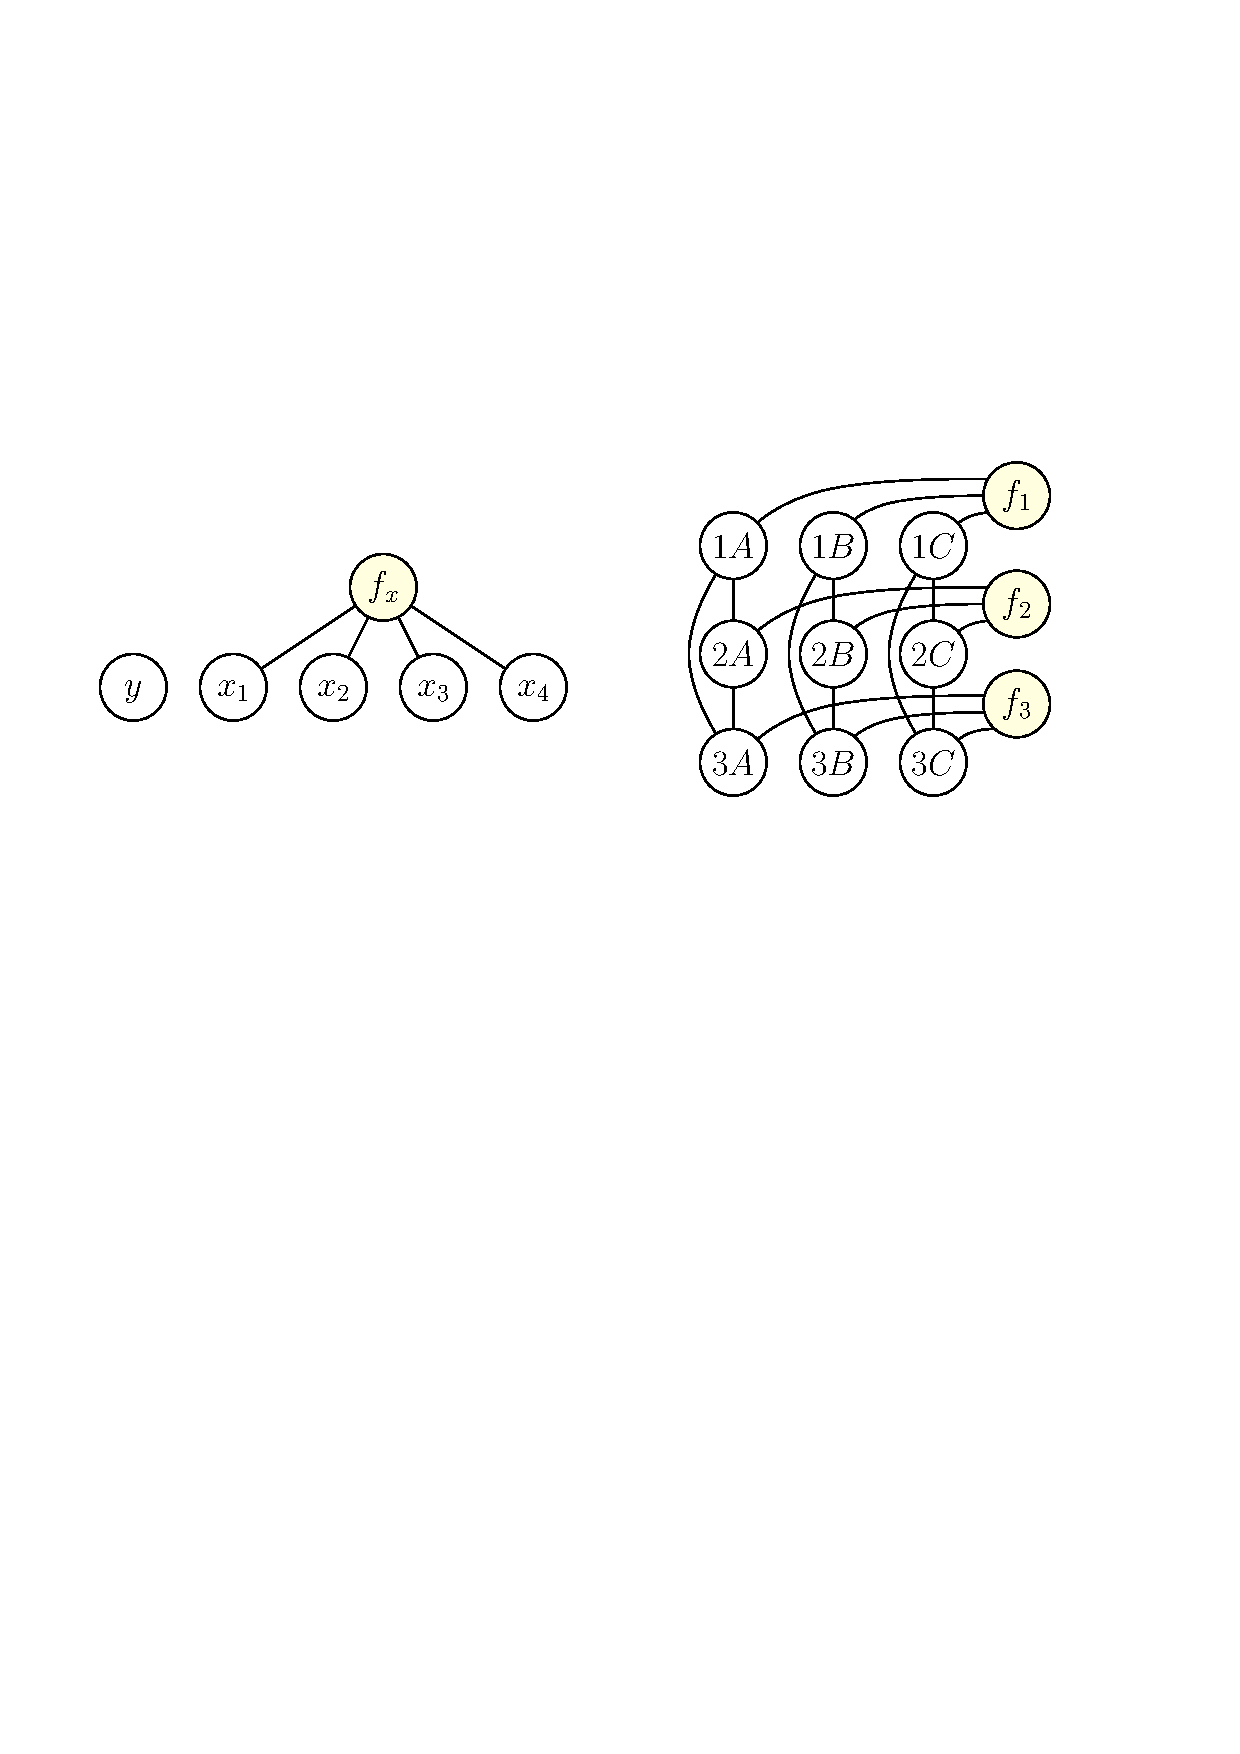
\includegraphics[width=.6\textwidth]{pictures/base-graph.pdf}
\caption{Base graph for the counterfeit coin problem with 4 coins (left) and\\
  for Mastermind with 3 pegs and 3 colours (right).}
\label{fig:base-graph}
\end{center}
\end{figure}
\end{example}

A more complicated example is the base graph for Mastermind with 3 pegs and 3 colours,
  shown on the right-hand side.
The vertices $f_1, f_2, f_3$ have separate labels, all other vertices are labelled ``variable''.
For simplicity, we leave out the symbol $x$ in the figure, e.g.
  write $1A$ instead of $x_{1A}$.\eqed

\begin{lemma}\label{lma:autobase}
Let  $\perm$ be an automorphism of $B$. Then $\perm|_\Var \in\symg$.
\end{lemma}

\begin{proof}
Let $\perm$ be an automorphism of $B$ and $(t, p)$ an experiment with a parametrization $p=p_1p_2...p_n$.
We show that there exists a $\perm$-symmetrical experiment to $(t, p)$.

Let $F_i\subseteq F$ be a set of mappings that are present in some outcome formula
  of $t$ with parameter $\$i$.
The vertices $f(p_i)$ for $f\in F_i$ form a clique in $B$ and so must the vertices
$\perm(f(p_i))$ for $f\in F_i$.
Since mappings $F$ have pairwise disjoint images, two variables $x_1, x_2$
  can be connected by an edge only if there is a symbol $k\in\Sigma$ and
  mappings $f,g\in F$ such that $f(k)=x_1$, $g(k)=x_2$.

We define $r_i$ as a symbol of $\Sigma$ that satisfies $f(r_i) = \perm(f(p_i))$ for some $f\in F_i$.
There always exists such $r_i$, because $f(p_i)$ cannot be mapped to a vertex that is not connected to $f$.
Due to the property above,
  if $f(r_i) = \perm(f(p_i))$ holds
  for \emph{some} $f\in F_i$,
  it holds for \emph{all} $f\in F_i$ and the definition is thus correct.

Now, consider the experiment $(t, r)$, where $r=r_1r_2,...r_n$.
All variables appearing directly in the parametrized formula are stabilized by $\perm$ and
  for all expressions $f(\$i)$ it holds $f(r_i)=\perm(f(p_i))$ by the construction of $r_i$,
  which means that $(t, r)$ is $\perm$-symmetrical to $(t, p)$. \qed
\end{proof}

\subsection{Experiment graph}

Let $\form\in\Form_X$ be a formula.
An \emph{$x$-rooted tree of $\form$}
  is a graph created from the syntax tree of $\form$
  by unification of the leaves that correspond to the same variables
  and adding a special vertex with label $x$ that is connected to the root
  of the syntax tree, i.e. to the top-level operator of $\form$.
Other vertices of the graph are labelled by their type (e.g. ``variable'', ``and-operator'', etc.)

In this construction, we need the trees of two formulas to be isomorphic if
  and only if the formulas are syntactically equivalent.
This clearly holds if all the operators are commutative.
As the only non-commutative operator is implication, we substitute
subformulas of the form $\form -> \formx$ with an equivalent formula $\formx \vee \neg\form$.

Let $B$ be the base graph for the given game, $\form\in\Formr$ some partial knowledge
  and $e$ an experiment.
The experiment graph $B_{\form, e}$ is constructed as follows.
\begin{itemize}
\item Begin with the graph $B$.
\item Add the ``knowledge''-rooted tree of $\form$.
\item For each outcome $\formx\in\outcome(e)$, add the ``outcome''-rooted tree of $\formx$.
\end{itemize}

\begin{theorem} \label{thm:isoequiv}
If $B_{\form, e_1}$ is isomorphic to $B_{\form, e_2}$, then
 $e_1 \expeq{\form} e_2$.
\end{theorem}

\begin{proof}
Let $\permx$ be the graph isomorphism of $B_{\form, e_1}$ and $B_{\form, e_2}$ and let
  $\perm = \permx|_\Var$, considered as a permutation of $\Var$.
Since $B$ is the vertex-induced subgraph of both $B_{\form,e_1}$ and $B_{\form, e_2}$ by
  the set of vertices $\Var\cupdot F$, $\perm$ is a member of $\symg$ by \autoref{lma:autobase}.

The isomorphism $\permx$ maps the only ``knowledge''-labelled vertex in the first graph
  to the only ``knowledge''-labelled vertex in the second graph,
  which implies the equivalence of the formulas, $\form^\perm \equiv \form$.
Similarly, ``outcome''-labelled vertices are mapped to ``outcome''-labelled vertices,
  which means that $\{\formx^\perm \| \formx\in\outcome(e_1)\} = \outcome(e_2)$.
This is sufficient for the experiments to be equivalent with respect to $\form$.
  \qed
\end{proof}

\begin{example}
Recall the running example of the counterfeit coin problem with four coins.
Base graph for the game was shown in \autoref{ex:cc-runbase}.
Let $\form=\init\wedge\neg(x_1\vee x_2)$ be the accumulated knowledge
  of the solving process $(12, =)$ and let $e$ be the experiment $3124$.
The experiment graph $B_{\form, e}$ is shown in \autoref{fig:exp-graph};
  Ex$_1$ denotes the $\exactlyk{1}$ operator.

Unfortunately, the graph for experiment 43 is clearly not isomorphic to this graph,
although the experiments are equivalent with respect to $\form$.
We address this problem in the following.\eqed

\begin{figure}[tt]
\begin{center}
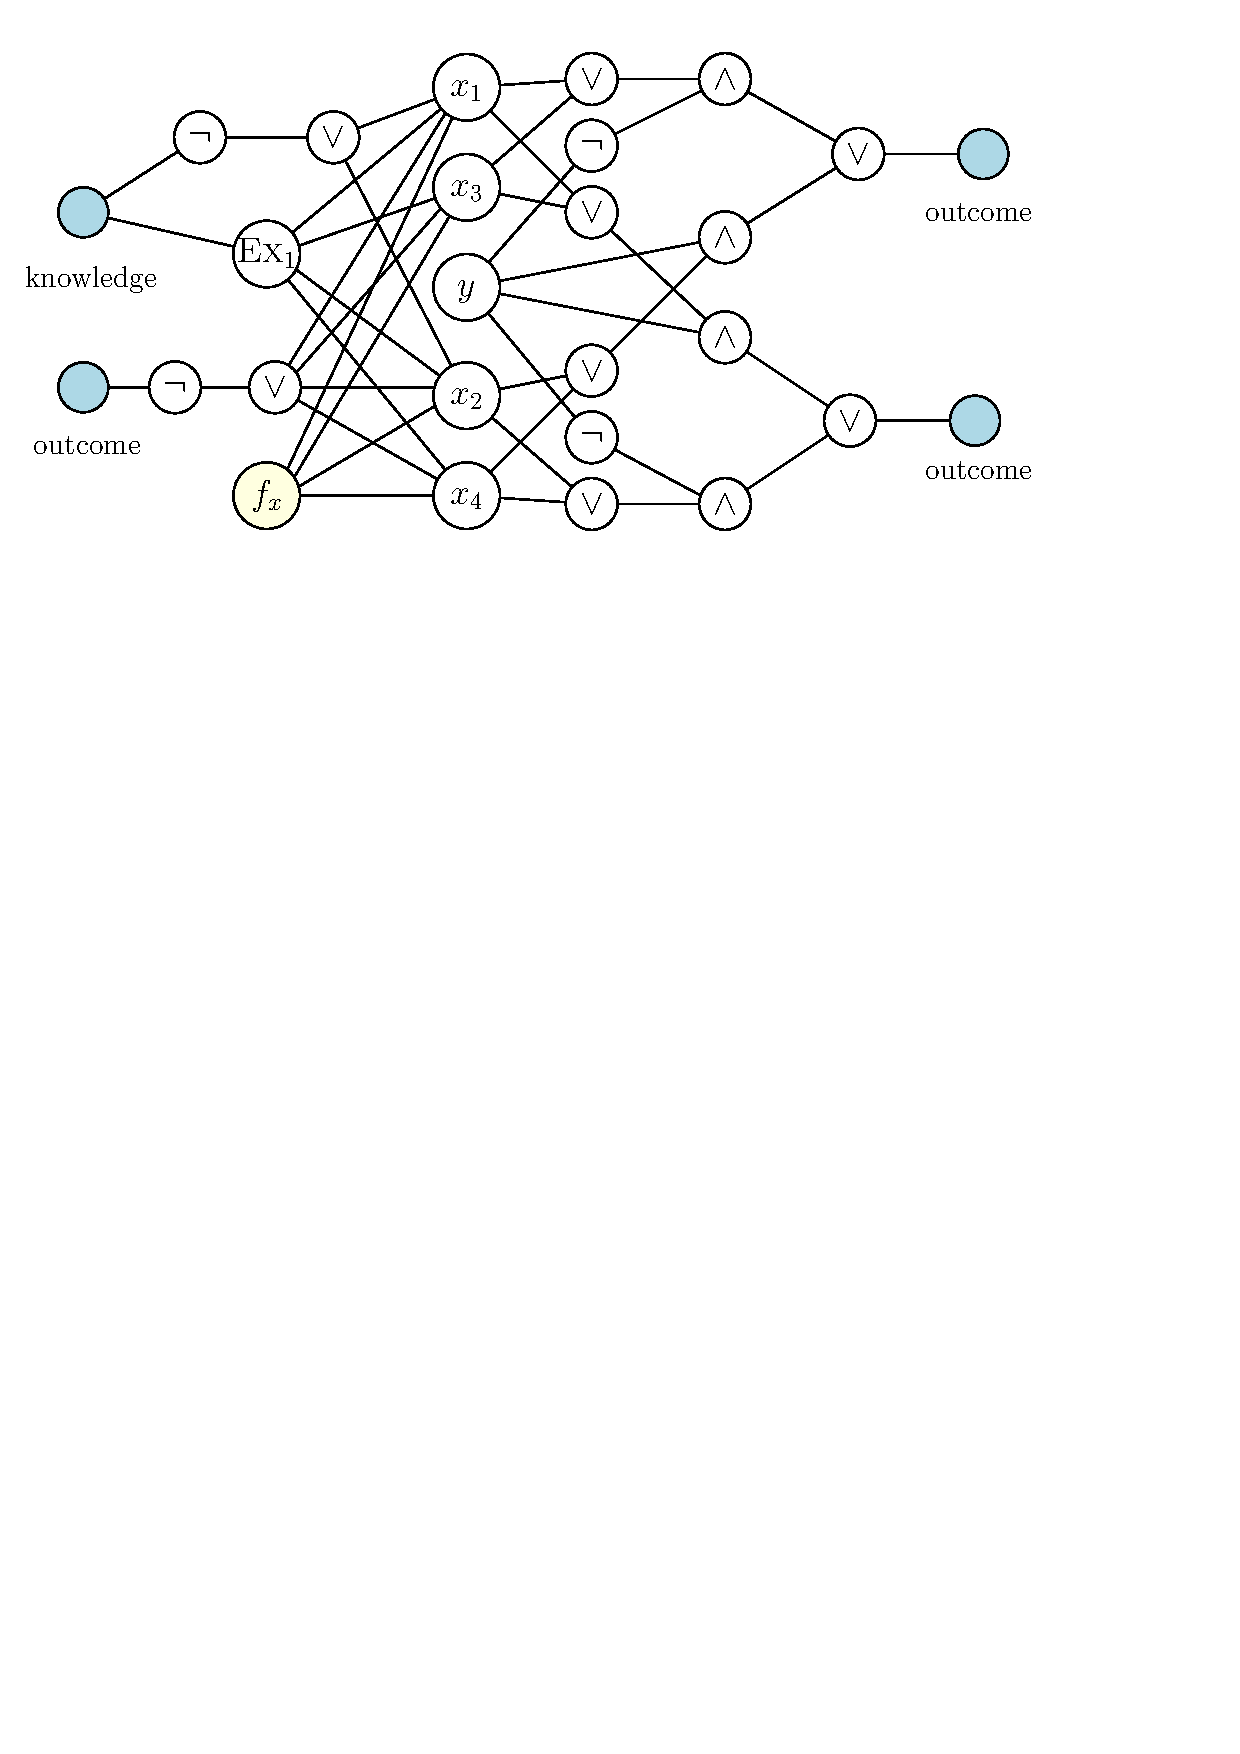
\includegraphics[width=.7\textwidth]{pictures/exp-graph.pdf}
\caption{Experiment graph for 3124 with knowledge $\init\wedge\neg(x_1\vee x_2)$.}
\label{fig:exp-graph}
\end{center}
\end{figure}
\begin{figure}[t]
\begin{center}
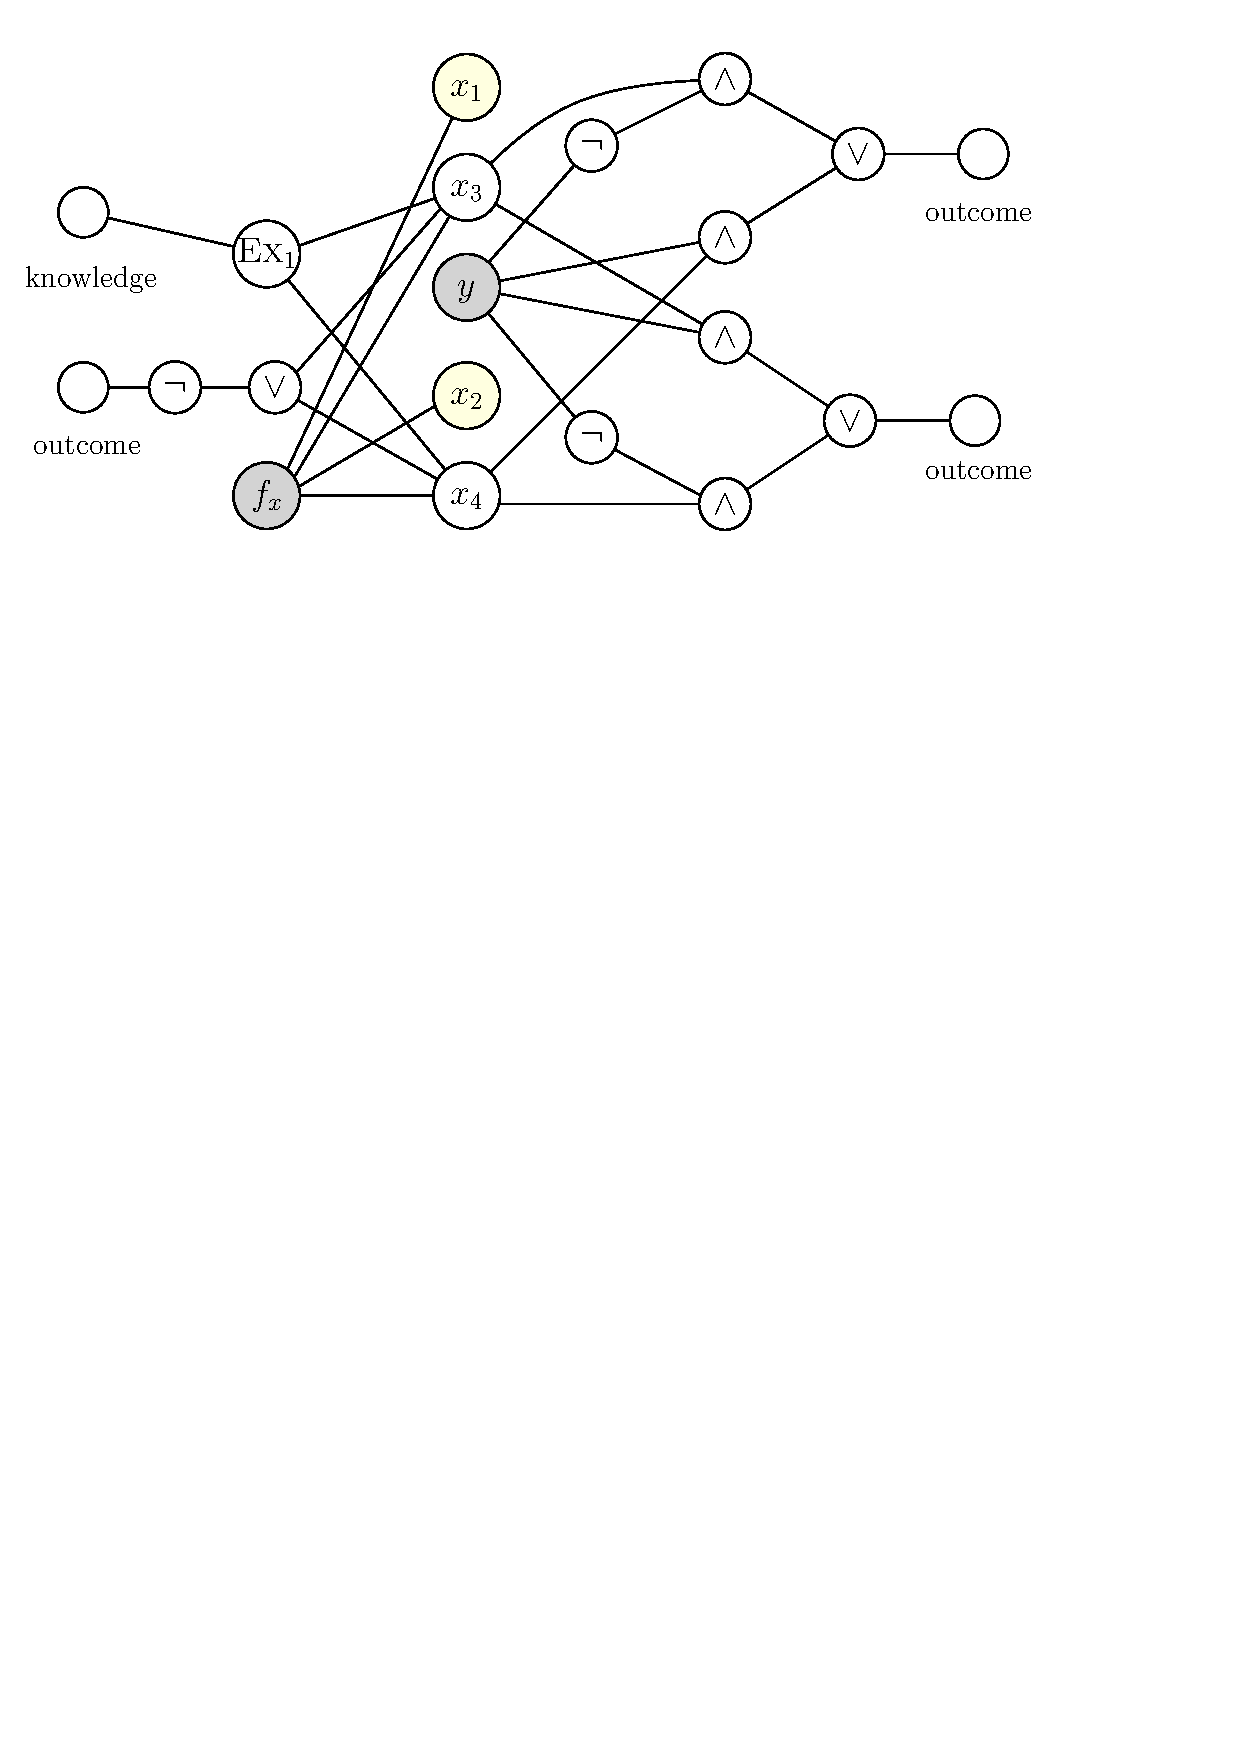
\includegraphics[width=.7\textwidth]{pictures/exp-graph-sim.pdf}
\caption{Simplified experiment graph for 3124 with knowledge $\init\wedge\neg(x_1\vee x_2)$.}
\label{fig:exp-graph-sim}
\end{center}
\end{figure}
\end{example}
\subsection{Improvement by fixed variables}

The previous example shows that the method explained above
  does not detect some basic equivalences.
To address the problem, we suggest the following improvement to the construction
  of $B_{\form, e}$.
\begin{enumerate} \itemsep 2pt
\item Compute fixed variables of the formula $\form$ using a SAT solver.
\item Simplify the formula $\form$ with the knowledge of its fixed variables.
\item Simplify the outcomes of $e$, formulas $\formx\in\outcome(e)$, with
  the knowledge of fixed variables of $\form$.
\item Construct the graph as described above.
\item Label the vertices corresponding to the fixed variables with the label ``false'' or ``true'',
  according to their fixed value.
\end{enumerate}

As the simplified formulas are equivalent to the original formulas,
\autoref{thm:isoequiv} also holds if the graphs $B_{\form, e_1}$, $B_{\form, e_2}$
are constructed with this approach.

\begin{example}
Let us apply the suggested improvement on the previous example.
The formula $\form = \init\wedge\neg(x_1\vee x_2)$ fixed variables
$x_1$ and $x_2$ to false.
\autoref{fig:exp-graph-sim} shows the constructed experiment graph
  after the simplification of the formulas.

The vertices $x_1$ and $x_2$ are now labelled ``false'' and are connected
  only to the vertex $f_x$.
Compare the structure with the graph in \autoref{fig:exp-graph}.
Note that the graph is now isomorphic to the graph of the experiment $43$.\eqed
\end{example}

\autoref{alg:noneqexp} describes the elimination of equivalent experiments with respect to a formula $\form$,
  which is a straightforward application of the method described in this section.
We assume there is a tool available for construction of the canonical labelling
  of a given graph,
  which is used to decide graph isomorphism.

\begin{algorithm}[!ht]
\caption{Elimination of equivalent experiments}
\KwIn{formula $\form$}
\KwOut{set $S\subseteq E$, such that $\forall e\in E \;\exists s \in S.\;e\expeq{\form}s$}
\label{alg:noneqexp}
\DontPrintSemicolon
$B <-$ construct the base graph for the game\;
$fixed <-$ compute fixed variables of $\form$ using a SAT solver\;
$\form' <- $ substitude values for fixed variables in $\form$ and simplify\;
Label the vertices in $B$ corresponding to the fixed variables with their fixed value\;
Add the ``knowledge''-rooted tree of $\form'$ to $B$\;
$S <- \emptyset$\;
$hash <- $ an empty hash table for graphs\;
\For{$e\in E$}{
  $B_e <- $ clone $B$\;
  \For{$\formx\in\outcome(e)$} {
    $\formx' <- $ substitude values for $fixed$ in $\formx$ and simplify\;
    Add the ``outcome''-rooted tree of $\formx'$ to $B_e$
  }
  $B_e <- $ canonize $B_e$\;
  \If{$B_e$ is not present in $hash$}{
    $hash$.insert($B_e$)\;
    $S <- S \cup \{e\}$\;
  }
}
\Return{$S$}
\end{algorithm}

\pagebreak
\section{Well-formed check}

Experiment equivalence can be used during the verification
  that a given game is well-formed, as stated by the following lemma.

\begin{lemma} \label{lma:well-formed}
  Let $S\subseteq E$ be a subset of experiments
  such that for every $e\in E$, there exists $s\in S$
   such that $e\expeq{\init}s$.
  If the formula $\init ==> \exactlyk{1}(\outcome(e'))$ is a tautology for
  all $s\in S$, then the game is well-formed.
\end{lemma}

\begin{proof}
Assume by contradiction that the game is not well formed, i.e.
  there is $e\in E$ and $v \in \Vals$ such that the number of
  formulas in $\outcome(e)$ satisfied by $v$ is not equal to one.

If $e\in S$, the formula $\init ==> \exactlyk{1}(\outcome(e'))$ is not
  satisfied by $v$. Contradiction.

Otherwise, there exists $s\in S$ such that $e\expeq{\init}s$, which means that
  there exists $\perm\in\Perm_\Var$ such that
$\{ \init\wedge\formx \| \formx\in\outcome(e) \} =
 \{ (\init\wedge\formx)^\perm \| \formx\in\outcome(s) \}$.
Since $\init ==> \exactlyk{1}(\outcome(s))$ is a tautology,
  the permuted formula
  $\init^\perm ==> \exactlyk{1}(\formx^\perm \| \formx\in\outcome(s))$
  is a tautology as well.
Therefore, exactly one formula from the set
 $ \{ (\init\wedge\formx)^\perm \| \formx\in\outcome(s) \}$
 is satisfiable and the same holds for
  $\{ \init\wedge\formx \| \formx\in\outcome(e) \}$,
 which implies that
 $\init ==> \exactlyk{1}(\outcome(e))$
 is a tautology. \qed
\end{proof}

\section{Analysis of one-step look-ahead strategies}

The following lemma gives us a right to disregard equivalent experiments
  during the analysis of some one-step look-ahead strategies.

\begin{lemma}
Let $f: 2^\Formr ->\Rset$ be a function such that
  $f(\formset) = f(\{\form^\pi \| \form\in\formset\})$ for any
  $\formset\subseteq\Formr$ and $\pi\in\Perm_\Var$ and
  let $\eord$ be a total order of $E$.
Let $\stg$ be the one-step look-ahead strategy with respect to $f$ and $\eord$, and
let $\form$ be a formula.
Suppose there are experiments $e_1$, $e_2$ such that $e_1\expeq{\form}e_2$ and $e_1\eord e_2$.
Then $\stg(\form) \not= e_2$.
\end{lemma}

\begin{proof}
If follows directly from \autoref{def:expeq} and the property of $f$ that
the function $f$ have the same value on $e_1$ and $e_2$, i.e.
\[f(\{\form\wedge\formx\| \formx\in\outcome(e_1)\}) =
 f(\{\form\wedge\formx\| \formx\in\outcome(e_2)\}).\]
Since $e_1 \eord e_2$, the strategy always prefers $e_1$ to $e_2$. \qed
\end{proof}

\vspace{-5mm}
\begin{algorithm}[ht]
\caption{Analysis of a one-step look-ahead strategy}
\label{alg:stganalysis}
\DontPrintSemicolon
\KwIn{function $f: 2^\Formr -> \Rset$, total order $\eord$ of $E$}
\KwOut{($w,a$), where $w$ and $a$ is the worst-case and the average-case number of experiments performed by the strategy}
$globalsum <- 0$\;
$globalmax <- 0$\;
\textsc{Analyse}($\init$, 1)\;
\Return$ (globalmax,\; globalsum \;/\; \numval\init)$\;\medskip
\setcounter{AlgoLine}{0}
\SetKwProg{optfun}{Function}{}{}
\optfun{\textsc{Analyse}\textnormal{($\form$, $depth$)}}{
$choice <- $None\;
$bestvalue <- \infty$\;
$S <- $ eliminate equivalent experiments by running \autoref{alg:noneqexp} on $\form$,
  where the experiments are considered in the order given by $\eord$\;
\For{$e\in S$ (variant 1) or $e\in E$ (variant 2)}{
  $value <- f(e)$
  \If{$value < bestvalue$} {
    $choice <- e$\;
    $bestvalue <- value$\;
  }
}
\For{$\formx\in\outcome(e)$}{
  \lIf{not $\SAT{\form\wedge\formx}$}{continue}
  \eIf{$\numval(\form\wedge\formx) = 1$}{
    $globalsum <- globalsum + depth$\;
    $globalmax <- max(globalmax, depth)$\;
  }{
    \textsc{Analyse}($\form\wedge\formx$, $depth + 1$)\;
  }
}
}{}
\end{algorithm}

Note that all one-step look-ahead strategies discussed in \autoref{sec:oslas}
  satisfy the condition of the lemma.
In general, any function based on satisfiability, the number of models and/or
  the number of fixed variables of the formulas will satisfy this requirement as
  these function are permutation independent.

A recursive approach for the analysis of one-step look-ahead strategies
  is shown in \autoref{alg:stganalysis}.
There are two options in line $5$ of the \textsc{Analyse} function.
The first is to use the algorithm to eliminate equivalent experiments and thus
  evaluate the strategy only on a subset of experiments.
The second is to go through all possible experiments.

In general, it cannot be said which variant is faster.
This depends on the ratio between the time
  needed for graph canonization and the
  time needed for strategy evaluation.

\section{Optimal strategy synthesis}

We suggest a method for worst-case and average-case
  optimal strategy synthesis based on backtracking.
In every state, we consider all possible experiments
  and compute the number of steps we need if we start with
  this experiment.
Our goal in this section is to prove that
  it is enough to analyse only one experiment from each equivalence class,
  as equivalent experiments give the same results.

\newcommand{\optval}{\kappa}
\newcommand{\optexp}{\varepsilon}
\newcommand{\optvale}{\kappa_\textrm{exp}}
\newcommand{\optexpe}{\varepsilon_\textrm{exp}}

First, let us define $\optval(\form)$ and $\optvale(\form)$ as
 the optimal number of experiments needed to reveal the secret code
  when starting with knowledge $\form$
  in the worst-case and in the average-case, respectively.
We can say that $\optval(\form)$ ($\optvale(\form)$) is
  the number of experiments of
  a worst-case (average-case) optimal strategy
  if we change the initial constraint of the game to $\form$.

Similarly, we define $\optval(\form, e)$ and $\optvale(\form, e)$ as
  the optimal number of experiment needed to reveal the secret code
  when starting with knowledge $\form$ and
  with $e$ as the first experiment.

There is an obvious relationship between $\optval(\form)$ and $\optval(\form,e)$
  and between $\optvale(\form)$ and $\optvale(\form,e)$.
For any $\form\in\Formr$,
\begin{equation}
\optval(\form) = \min_{e\in\Exp}\optval(\form, e),\textrm{ and }
\hspace{1cm}
\optvale(\form) = \min_{e\in\Exp}\optvale(\form, e).
\label{opttriv}
\end{equation}

Further, we can compute $\optval(\form, e)$ and $\optvale(\form, e)$
  from the optimal values for the subproblems after the first experiment.
These relationships are based on the definitions of the worst-case
  and average-case number of experiments of a strategy
  ($\lenmax{\stg}$ and $\lenexp{\stg}$).
For any $\form\in\Formr$ and $e\in E$,
\begin{align}
\optval(\form, e) &= \left\{\begin{array}{ll}
 0 & \textrm{ if }\numval{\form} = 1, \\
 \infty & \textrm{ if }\exists\formx\in\outcome(e).\; \form\wedge\formx\equiv\form, \\
 1 + \max_{\formx\in\outcome(e)}\optval(\form\wedge\formx) &
 \textrm{ otherwise. }
\end{array}\right.\label{optval}\\
\optvale(\form, e) &= \left\{\begin{array}{ll}
 0 & \textrm{ if }\numval{\form} = 1, \\
 \infty & \textrm{ if }\exists\formx\in\outcome(e).\; \form\wedge\formx\equiv\form, \\
 1 + \frac{\sum_{\formx\in\outcome(e)}\numval{(\form\wedge\formx)}\cdot\optvale(\form\wedge\formx)}{\numval{\form}} &
 \textrm{ otherwise. }
\end{array}\right.\label{optvale}\\
\end{align}

Let us now define the sets of optimal choices in a state.
For a $\form\in\Formr$, we define
\begin{align*}
\optexp(\form) &= \{ e\in E \| \forall e'\in E.\; \optval(\form, e) <= \optval(\form, e') \},\textrm{ and }\\
\optexpe(\form) &= \{ e\in E \| \forall e'\in E.\; \optvale(\form, e) <= \optvale(\form, e') \}.
\end{align*}

The following lemma is a straightforward consequence of the definitions of $\optval$ and~$\optexp$.

\begin{lemma}
If $\stg$ is a strategy such that $\stg(\form)\in\optexp(\form)$ for every $\form\in\Formr$,
 $\stg$ is worst-case optimal.
Similarly, if $\stg'$ is a strategy such that $\stg'(\form)\in\optexpe(\form)$ for every $\form\in\Formr$,
 $\stg'$ is average-case optimal.
\end{lemma}

Now, we are ready for the main theorem of this section.
The first part gives us a right to compute the value of $\optval$
  on symmetrical formulas only once.
The second part
  allows us to consider
  only one experiment from
  each equivalence class of $E/\expeq{\form}$
  in every state.
The exact algorithm for optimal strategy synthesis
  with further optimizations is described in \autoref{s:cobra-modes}.

\begin{theorem}
For every $\form\in\Formr$,
\begin{enumerate}
\item $\optval(\form) = \optval(\form^\perm)$ and $\optvale(\form) = \optvale(\form^\perm)$ for all $\perm\in\symg$, and
\item if $e_1\expeq{\form} e_2$, then $e_1\in\optexp(\form) \Leftrightarrow e_2\in\optexp(\form)$ and
  $e_1\in\optexpe(\form) \Leftrightarrow e_2\in\optexpe(\form)$.
\end{enumerate}
\end{theorem}

\begin{proof}
The proof for the worst case ($\optval, \optexp$)
  and for the average case ($\optvale, \optexpe$) is exactly the same,
  so we show only the proof for the worst case.

Since $\perm\in\symg$, there exists a $\perm$-symmetrical experiment $e^\perm$
  to $e$ for every $e\in E$.
Recall that $\outcome(e^\perm) = \{ \formx^\perm \| \formx\in\outcome(e)\}$.
We show by induction on the number of models of $\form$
  that $\optval(\form, \exp) = \optval(\form^\perm, \exp^\perm)$,
  which is sufficient for the first part.

As $\numval{\form} = \numval{\form^\perm}$, the statement follows directly from
  (\refeq{opttriv}) and (\refeq{optval}) for formulas with one model.
For the induction step, observe that
  $\numval(\form^\perm \wedge \formx^\perm) = \numval(\form\wedge\formx)$
  and, by the induction hypothesis,
  $\optval(\form^\perm \wedge \formx^\perm) = \optval(\form\wedge\formx)$
  if $\form \not\equiv \form\wedge\formx$.
The statement now follows from (\refeq{optval})
  as the right sides are equal.

For the second part, it suffices to prove that
  $\optval(\form, e_1) = \optval(\form, e_2)$.
As the experiments are equivalent, there exists a permutation $\perm\in\symg$,
 such that
 $\{\form\wedge\formx \|\formx\in\outcome(e_1)\} =
 \{(\form\wedge\formx)^\perm \|\formx\in\outcome(e_2)\}$.
The equation now follows from (\refeq{optval}) and the facts that
 $\numval\form=\numval\form^\perm$ and $\optval(\form) = \optval(\form^\perm)$
 (proven in the first part). \qed
\end{proof}

A recursive algorithm for computation of the value
  of the worst-case and the average-case optimal strategy,
  $\optval(\form)$ and $\optvale(\form)$ is shown in \autoref{alg:acopt}.
The lines marked with [W] applies only to the worst case,
  the lines marked with [A] applies only to the average case.

The algorithm makes use of the first part of the theorem by caching the results and
  checking that the function has not yet been called on the same or a symmetrical formula
  in the begging.
This is done similarly to the symmetry detection described in \autoref{sec:expeq}.
We construct the base graph of the game, add the ``knowledge''-rooted tree of $\form$,
  canonize the graph and compare with the graphs we have already seen.

Apart from the formula $\form$, the recursive function takes another argument, $opt$,
  which is used for branch pruning in the computation of the worst-case optimal strategy.
The value of $opt$ is an upper bound on $\optval(\form)$.
Therefore, if we are sure that $\optval(\form, e) > opt$ for a given experiment $e$,
  we can continue with the analysis of another experiment.
A lower bound on $\optval(\form, e)$ can be computed using \autoref{lma:lbound}.
The initial value of $opt$ should be $\infty$ or any known upper bound on $\optval(\init)$.

\begin{algorithm}[ht]
\caption{Computation of the worst-case (W) and the average-case~(A) optimal number of experiments.}
\label{alg:acopt}
\DontPrintSemicolon
\SetKwProg{optfun}{Function}{}{}
\optfun{\textsc{Optimum}\textnormal{($\form$, $opt$)}}{
\lIf{$\numval{\form} = 1$}{\Return{0}}
Compute a canonical form of $\form$. If the function has already been called
  on $\form$ or a symmetrical formula, use the cached result. \;
[W] $ lb <- \textsc{LowerBound}(\form)$\;
[W] \lIf{$lb > opt$}{\Return{$\infty$}}
$S <- $ compute a subset of experiments such that
  $e\in E ==> \exists e'\in S.\;e\expeq{\form}e'$\;
% $ b <- $ maximal number of satisfiable outcomes of an experiment in $S$\;
% $ lb <- \textsc{LowerBound}(\form, b)$\;
% \lIf{$lb > opt$}{\Return{$\infty$}}
\For{$s\in S$, ordered by $\max_{\formx\in\outcome(s)}\numval(\form\wedge\formx)$}
{
  \lIf{only one of $\form\wedge\formx$, $\formx\in\outcome(s)$ is satisfiable}{continue}
  $ val <- 0 $\;
  \For{$\formx\in\outcome(s)$} {
    \If{$\SAT{\form\wedge\formx}$}{
[W] $val <- \max( val, 1 + \textsc{Optimum}(\form\wedge\formx,\; opt-1))$\;
[A] $val <- val + \numval(\form\wedge\formx)\cdot
      (1 + \textsc{Optimum}(\form\wedge\formx,\; opt-1))$\;
    }
  }
  [A] $val <- val \;/\; \numval(\form)$\;
  \lIf{$val < opt$}{$opt <- val$}
}
Store the information that the value for $\form$ is $opt$\;
\Return{$opt$}
}{}
\end{algorithm}

Note that the order of the experiments in line 7
  is not necessary for the correctness of the algorithm.
The idea here is to try to find a good experiment as soon as possible,
  so that we can prune some branches on the lower bound check.

